%Root main.tex
%---------------------------------------------------------------------------
%第2章　aaa
%---------------------------------------------------------------------------

\chapter{実機の基礎検証}
\label{chap:基礎検証}

\section{実機実装}
\subsection{ゲイン近似}
デッドビート制御ゲインの演算式に行列指数関数$e^{AT}$があり，式(\ref{for:SRDB式})のままでFPGAに書き込むと，膨大な演算量が発生し，大量のFPGAロジックセルを消費しまうため，拡張機能向けのロジックセル量が少なくなる．FPGAの演算量を低減するように，制御ゲインの結果をプロットし，近似式を求める．表\ref{for:GainPlot}に制御ゲインプロットする際の条件を示す．プロットした制御ゲイン$G^{-1}$,$G^{-1}F$それぞれを図\ref{fig:invG}，図\ref{fig:invGF}に示す．
\begin{table}[h]
 \center
 \caption{制御ゲインプロット用の条件}
 \label{for:GainPlot}
 \small
 \begin{tabular}{c|c} \hline \hline
  パラメータ定義		 & 値 		\\ \hline
  $d$軸インダクタンス($L_d$)[mH] & 6.9454	\\ \hline
  $q$軸インダクタンス($L_q$)[mH] & 8.8403	\\ \hline
  巻き線抵抗($R_L$)[$\Omega$]	 & 1.44		\\ \hline  
  キャリア周波数[Hz]		 & 5k		\\ \hline
  サンプリング周波数[Hz]	 & 1M		\\ \hline
  回転速度($N$)[rpm]		 & 0\textasciitilde2000		\\ \hline
 \end{tabular}
\end{table}
\begin{figure}[h]
 \center
 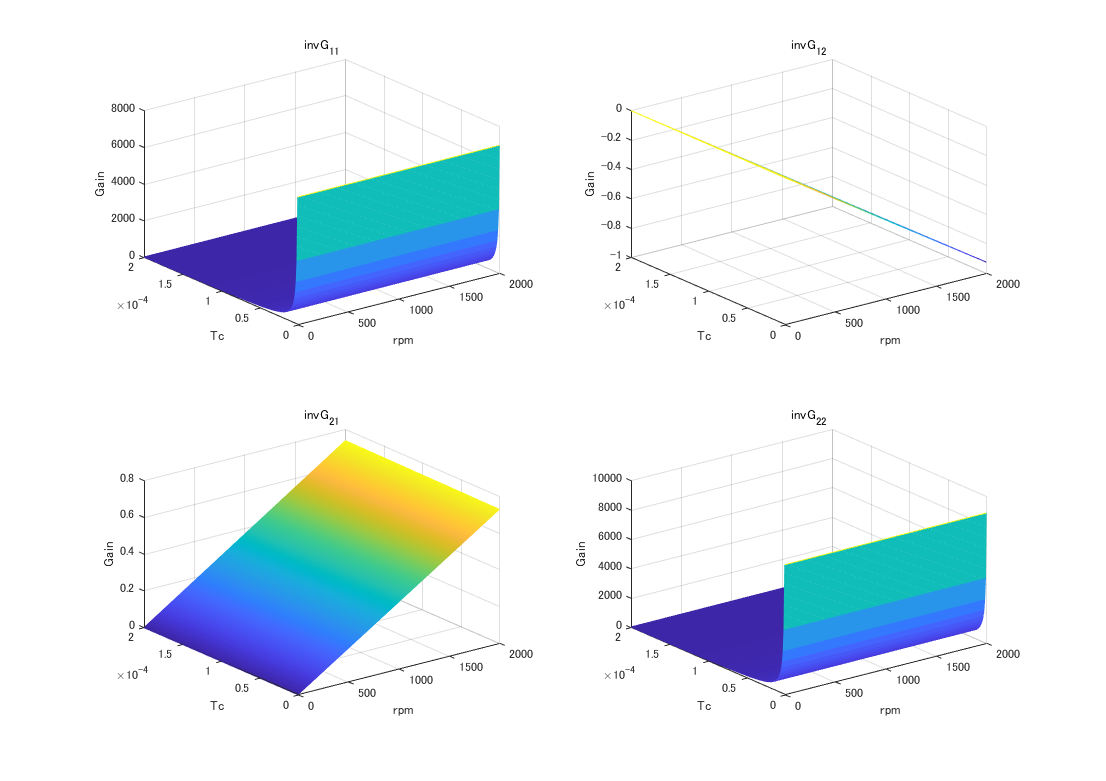
\includegraphics[width=120mm]{image/chapter5/invG.png}
 \caption{制御ゲイン$G^{-1}$}
 \label{fig:invG}
\end{figure}
\begin{figure}[h]
 \center
 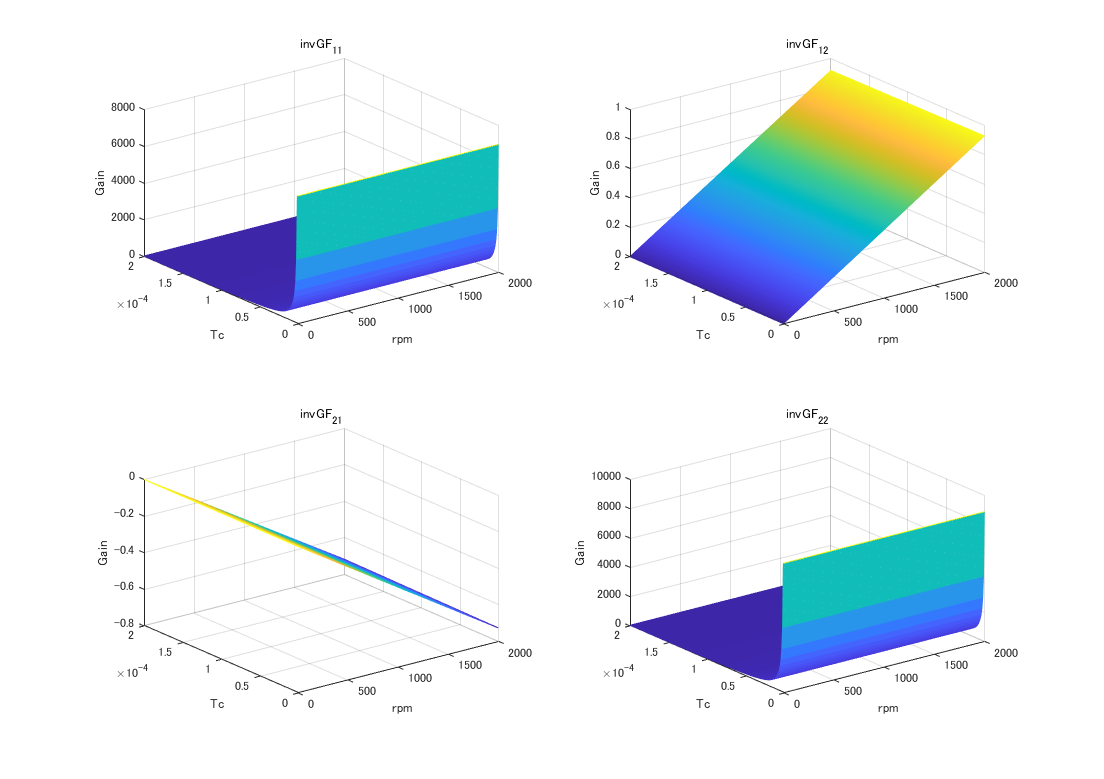
\includegraphics[width=120mm]{image/chapter5/invGF.png}
 \caption{制御ゲイン$G^{-1}F$}
 \label{fig:invGF}
\end{figure}

図\ref{fig:invG},\ref{fig:invGF}より，ゲイン$G^{-1}_{11}$,$G^{-1}_{22}$,$G^{-1}F_{11}$,$G^{-1}F_{22}$の変化はモータの回転数に依存しないことがわかったため，モータ回転を考慮しないで近似する．また，$T_c$が小さくなるとともに，ゲイン$G^{-1}_{11}$,$G^{-1}_{22}$,$G^{-1}F_{11}$,$G^{-1}F_{22}$が大きくなり，0\textasciitilde50$\mu s$の間，指数変化とみなされる．$\mu s$で急激な変化が起きる場合，FPGA演算にはオーバーフローが生じやすくなる．それ故，リミッタを設けて，上限値を上回ったら，上限値を出力する．今回，50$\mu s$のところにゲインリミッタを入れる．図\ref{fig:no_omega_Gain}にリミッタありおよびモータ回転を考慮しないゲイン$G^{-1}_{11}$,$G^{-1}_{22}$,$G^{-1}F_{11}$,$G^{-1}F_{22}$を示す．
\begin{figure}[h]
 \center
 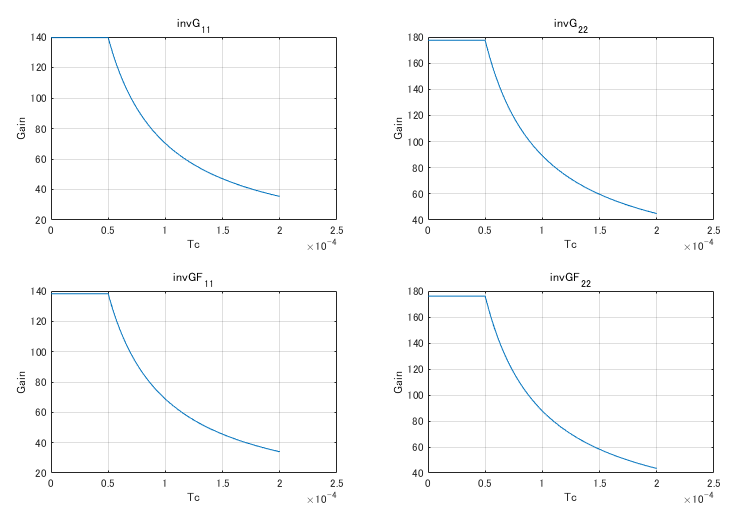
\includegraphics[width=105mm]{image/chapter5/limit_Gain.png}
 \caption{モータ回転を考慮しないゲイン}
 \label{fig:no_omega_Gain}
\end{figure}

$G^{-1}$,$G^{-1}F$の近似式は以下となる．
\begin{eqnarray}
 G^{-1}\left\{
 \begin{aligned}
    &G^{-1}_{11}=139.629(0<T_c<50\mu s)\\
    &G^{-1}_{11}=\frac{0.006944}{T_c}+0.7306(50<T_c<200\mu s)\\
    &G^{-1}_{12}=0.00287-0.0004657\omega-28.56T_c\\
    &G^{-1}_{21}=-0.00226-0.0003659\omega+22.44T_c\\
    &G^{-1}_{22}=177.527(0<T_c<50\mu s)\\
    &G^{-1}_{22}=\frac{0.008836}{T_c}+0.7283(50<T_c<200\mu s)
 \end{aligned}
 \right.
 \label{for:invG}
\end{eqnarray}
\begin{eqnarray}
 G^{-1}F\left\{
 \begin{aligned}
    &G^{-1}F_{11}=138.189(0<T_c<50\mu s)\\
    &G^{-1}F_{11}=\frac{0.00694}{T_c}-0.7094(50<T_c<200\mu s)\\
    &G^{-1}F_{12}=0.00287+0.00046\omega-28.56T_c\\
    &G^{-1}F_{21}=-0.00226-0.0003614\omega+22.44T_c\\
    &G^{-1}F_{22}=176.087(0<T_c<50\mu s)\\
    &G^{-1}F_{22}=\frac{0.008836}{T_c}-0.7117(50<T_c<200\mu s)
 \end{aligned}
 \right.
 \label{for:invGF}
\end{eqnarray}

式(\ref{for:invG}),(\ref{for:invGF})における$T_c$の初期値はキャリア周期と同じであり，1サンプリング毎にAD変換周期である1$\mu$sずつ減少させる．$\omega$はモータ角速度である．
\subsection{HDLコード生成}
開発周期の短縮、デバッグ作業の簡素化、コードのトレーサビリティ、早期検証などのことを実現するため，MATLAB/HDL Coderツールを利用する．HDLコード生成手順は主にSimulinkにおいてコードを生成するための回路作成、回路のシミュレーションおよび結果検証、固定小数点ツールでデータ型の最適化、HDLコード生成四つがある．コード生成のSimulinkを図\ref{fig:HDL_Simulink}に示す．
\begin{figure}[h]
 \center
 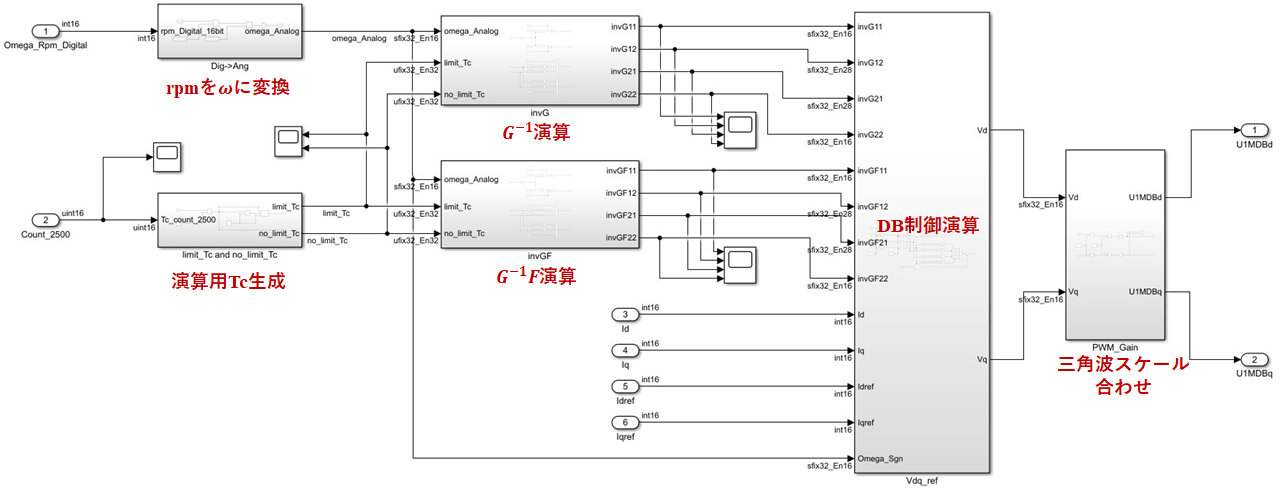
\includegraphics[width=135mm]{image/chapter5/HDL_Simulink.png}
 \caption{HDLコード生成のSimulinkモデル}
 \label{fig:HDL_Simulink}
\end{figure}

HDLコード生成回路による演算したゲインが正しいことを検証するため，シミュレーションを行い，図\ref{fig:Simulink_Gain}にシミュレーション波形示す．ただし，シミュレーション条件は表\ref{for:GainPlot}と同じである．

\begin{figure}[h]
 \center
 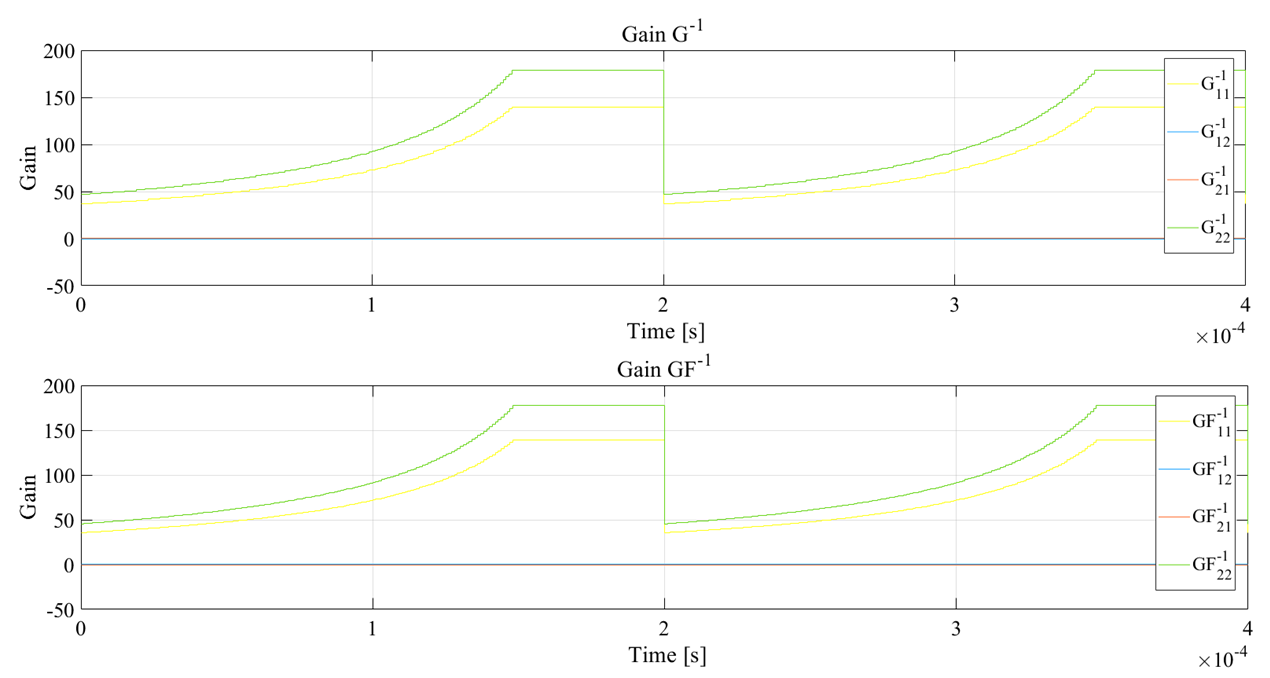
\includegraphics[width=130mm]{image/chapter5/HDL_Gain.png}
 \caption{近似ゲインの検証波形}
 \label{fig:Simulink_Gain}
\end{figure}

波形より，HDLコード生成回路による演算したゲインはゲイン近似で求めた結果が一致しており，回路が正しいと考えられる．シミュレーションを行う際，double型データを用いたが，FPGAに扱っているデータは固定小数点型のため，図\ref{fig:Fitting Tool}の固定小数点ツールによるデータ変換を行う．データ範囲も同時表示されるため，オーバーフロー、アンダーフローを無くすようにデータ型を調整する．
\begin{figure}[h]
 \center
 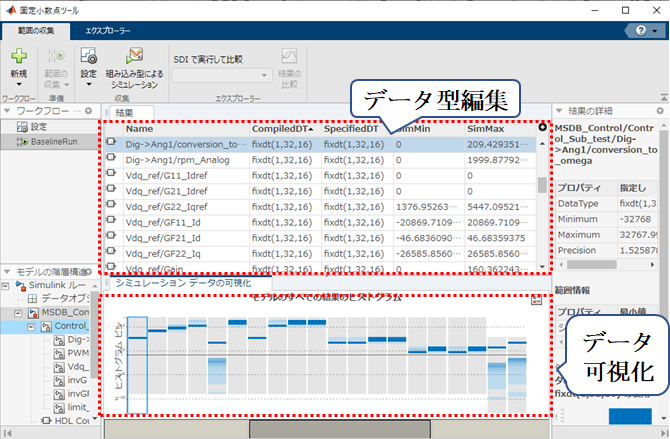
\includegraphics[width=120mm]{image/chapter5/Curve_Fitting_Tool.png}
 \caption{固定小数点ツール}
 \label{fig:Fitting Tool}
\end{figure}

調整したデータ型をSimulinkに適応し，HDL Coderツールでコード生成を行う．図\ref{fig:MSDB_HDL}に生成したHDLモジュール構成を示す．
\begin{figure}[h]
 \center
 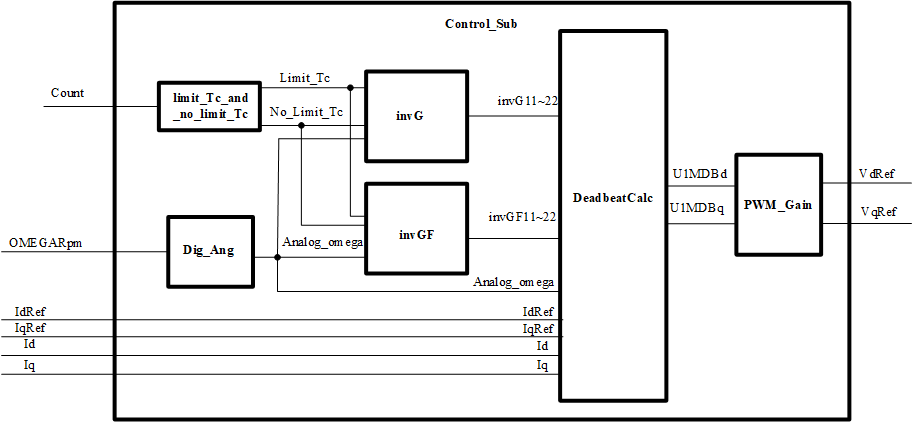
\includegraphics[width=120mm]{image/chapter5/MSDB_HDL.png}
 \caption{生成したHDLモジュール構成}
 \label{fig:MSDB_HDL}
\end{figure}

図\ref{fig:MSDB_HDL}に示しているように，$T_c$場合分けモジュール・回転速度演算モジュールはホールドあり、なし$T_c$と$rad/s$である回転速度を算出し，ゲイン演算モジュールに渡す．操作量演算モジュールは実電流、指令電流および制御ゲインを受信し，$dq$軸操作量を出力する．操作量と三角波スケールを合わせるため，正規化モジュールを利用する．


\newpage
\section{実機結果}
\subsection{実機構成および検証条件}
生成したHDLコードの正確性を検証する実機構成を図\ref{fig:real systeam}に示す．

\begin{figure}[h]
 \center
 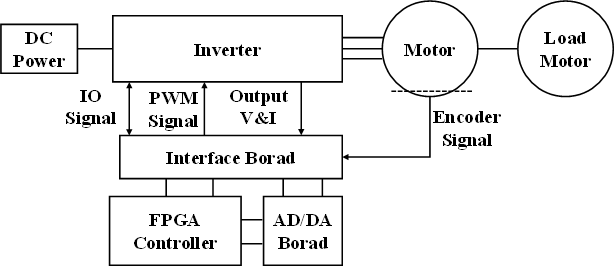
\includegraphics[width=110mm]{image/chapter5/real_systeam.png}
 \caption{コード検証の実機構成}
 \label{fig:real systeam}
\end{figure}

直流電源はインバータに200V電圧を提供する．インバータにおけるスイッチング素子はFPGAから送信されたPWM信号によってON/OFFし，三相交流を出力する．エンコーダで計測した角速度および回転角がインタフェースボードを通って，FPGAコントローラに送信される．電流センサによる取得した電流がインタフェースボード、AD変換基板を介してFPGAコントローラにフィードバックする．HDL開発ソフトQuartusを用いて生成したコードをFPGAコントローラに実装する．実機検証の条件を表\ref{for:実機条件}に示す．

\begin{table}[h]
 \center
 \caption{制御ゲインプロット用の条件}
 \label{for:実機条件}
 \small
 \begin{tabular}{c|c} \hline \hline
     条件の定義		 & 値 		\\ \hline
     回転速度($N$)[rpm]	 & 200		\\ \hline
     キャリア周波数[Hz]		 & 5k	\\ \hline
     サンプリング周波数[Hz]	 & 1M		\\ \hline
     $d$軸指令電流($i_{dref}$)[A]	 & 0		\\ \hline
     $q$軸指令電流($i_{qref}$)[A]	 & 0→1.5	\\ \hline
 \end{tabular}
\end{table}

\newpage
\subsection{実機波形}
図\ref{fig:MSDB_Real_Ans}にMSDB制御の実機波形，図\ref{fig:MSDB_Real_Big}にdq軸立ち上がり部分の拡大を示す．
\begin{figure}[h]
 \center
 \includegraphics[width=140mm]{image/chapter5/Real_dq.png}
 \caption{MSDB制御の$dq$軸電流}
 \label{fig:MSDB_Real_Ans}
\end{figure}
\begin{figure}[h]
 \center
 \includegraphics[width=140mm]{image/chapter5/Real_dq_big.png}
 \caption{$dq$軸電流の拡大図}
 \label{fig:MSDB_Real_Big}
\end{figure}

$dq$軸実電流波形より，$d$軸実電流が指令電流0Aに到達するまでの時間は約202$\mu s$であり，その後，目標電流0Aに追従している．$q$軸実電流が目標電流1.5Aに到達するまでの時間は約200$\mu$sである．また，$d,q$軸実電流それぞれのリップル率は11.3$\%$,16.4$\%$であることがわかる．$dq$軸電流はいずれも1キャリア程度で指令値に追従したため，実機結果とシミュレーション結果が一致しており，生成したコードの正確性を検証できた．

% 図
% \begin{figure}[htb]
%  \begin{center}
%  \includegraphics[width=50mm]
%  {image/image1}
%  \caption{}
%  \label{fig:}
%  \end{center}
% \end{figure}

% 表
% \begin{table}[htb]
%  \centering
%  \caption{}
%  \label{tab:}
%  \begin{tabular}{c|c}
%   \hline\hline
%   &\\ \hline
%   &\\ \hline
%  \end{tabular}
% \end{table}

% 式
% \begin{eqnarray}
%  a=b \nonumber \\
%  c=d \label{for:}
% \end{eqnarray}

% ソース
% \lstinputlisting[
%   caption=, 
%   label=list:
% ]
% {source/code1}